\subsection{Numerical Differentiation}
\label{subsec:numeric}

\begin{frame}
\frametitle{Numerical Differentiation}
\framesubtitle{From First-Principles}
%
\colorbox{green!10}{\vbox{
%
\begin{center}
%
Estimate the gradient by looking at the rate of change.
%
\end{center}
%
}}
%
\begin{itemize}
%
\item Finite Difference: $\color{m1} f'(x) \approx \frac{f(x+h)-f(x)}{h} $
%
\item Central Difference: $\color{m1} f'(x) \approx \frac{f(x+h)-f(x-h)}{2h}$
%
\item Imaginary Difference: 
         $\color{m1} f'(x) \approx \mathrm{Im}\left(\frac{f(x+ih)}{h}\right)$
%
\end{itemize}
%
For $\color{m1}h<\epsilon x$, where $\color{m1}\epsilon$ is the machine
precision, these approximations become zero. 
%
Thus $\color{m1}h$ has to be chosen with care.
%
\end{frame}

\begin{frame}
\frametitle{Numerical Differentiation}
\framesubtitle{Imaginary Differentiation Error}
%
The graph shows the error in approximating the derivative for
$\color{m1}f(x)=e^x$ as a function of $\color{m1}h$.
%
\begin{center}
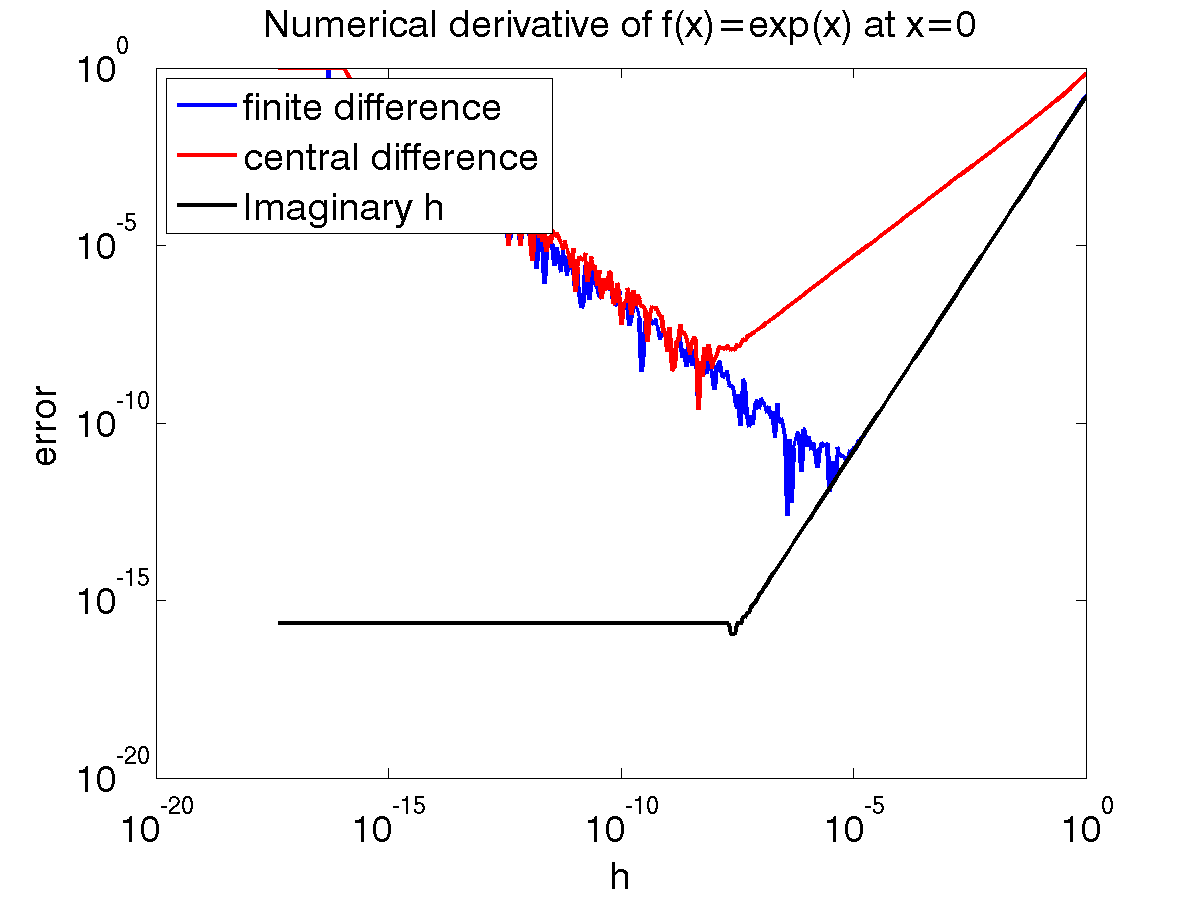
\includegraphics[height=0.5\textwidth]{figs/findifferror2}
\end{center}
%
\end{frame}
